%%%%%%%%%%%%%%%%%%%%%%%%%%%%%%%%%%%%%%%%%%%%%%%%%%%%%%%%%%%%%%%%%%%%%%%%%%%%%%%


\chapter{RESULTADOS}

A Figura \ref{fig:resume} exibe as funções de Cantor analisadas nessa seção e seus respectivos espectros. Os demais resultados desta seção corespondem aos espectrogramas gerados, e estão separados pelo valor do parâmetro \texttt{seed} e tamanho da janela. As Figuras exibem os resultados das seis janelas implementadas. O eixo horizontal das figuras corresponde ao intervalo [0,1] e possui o rótulo ``tempo'' (ou ``t'') para manter analogia à análise de um sinal.

\begin{figure}[ht!]
	%\caption{Funções de Cantor analisadsa neste estudo e seus espectros de Fourier.}
	\vspace{1mm}	
	\begin{center}
		\resizebox{9cm}{!}{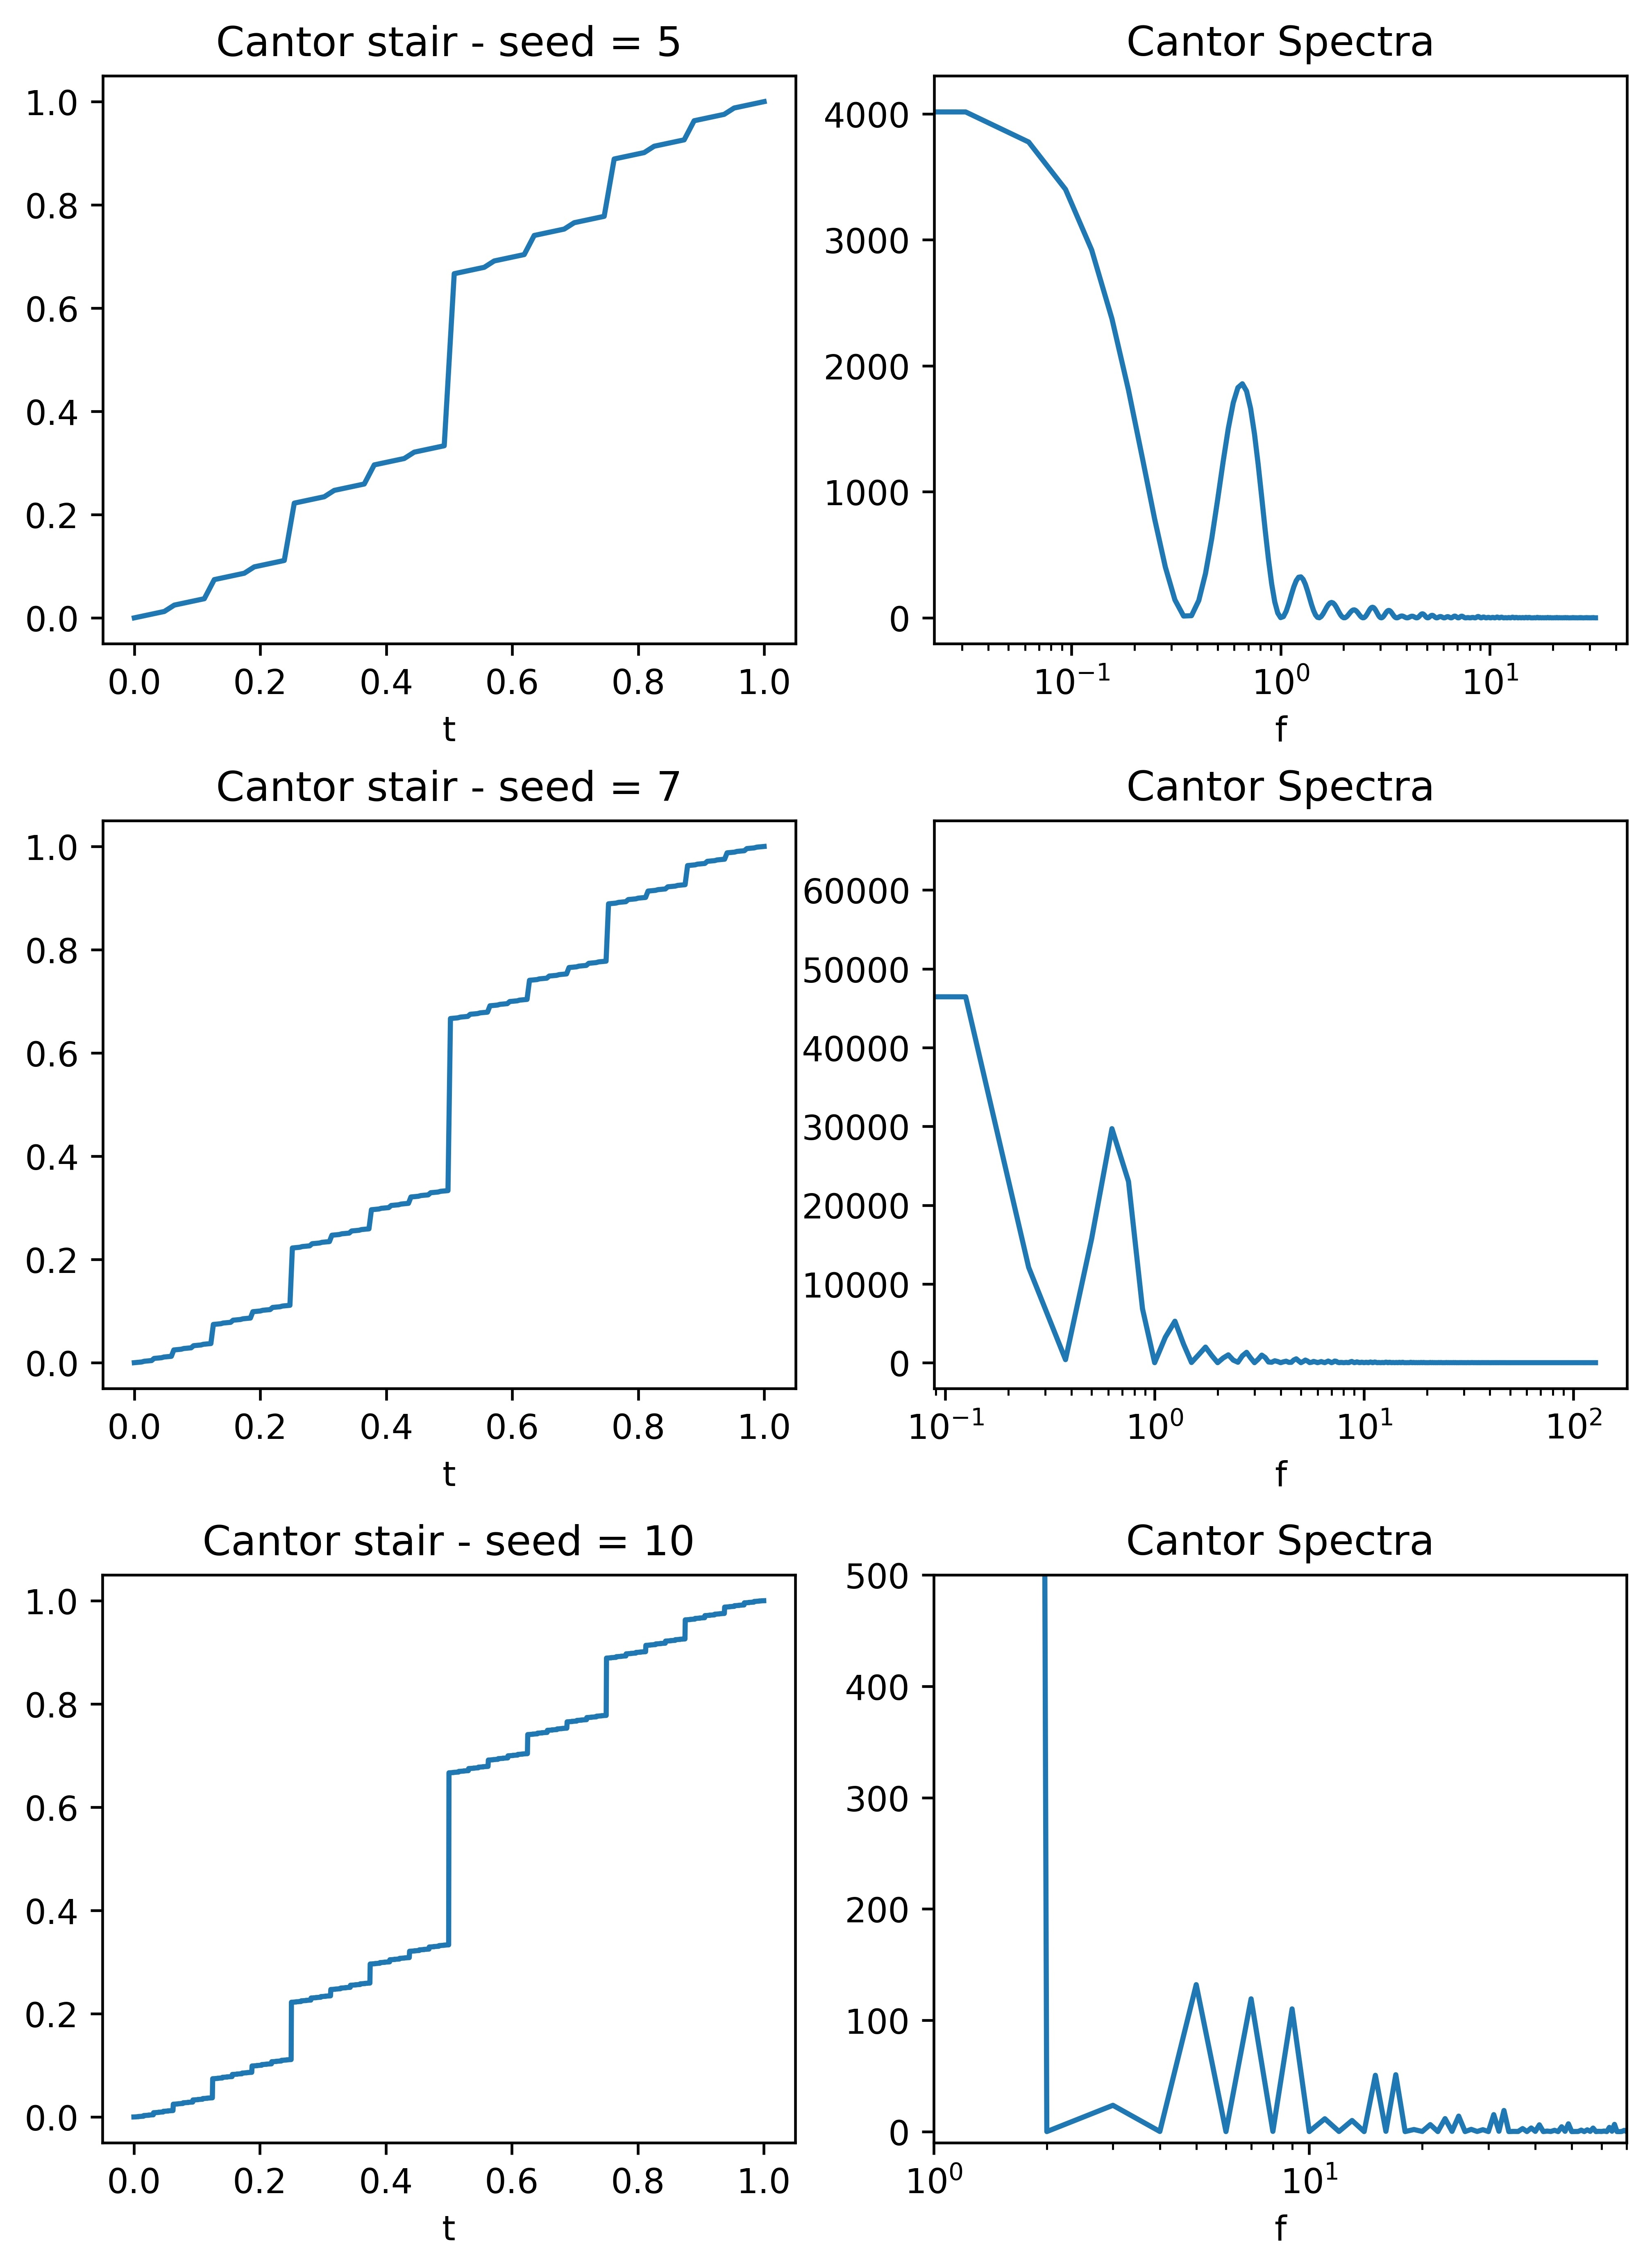
\includegraphics{../Figuras/cantor_figs.jpg}}
	\end{center}
	\vspace{1mm}	
	\caption{Funções de Cantor analisadsa neste estudo e seus espectros de Fourier. Observa-se que, quanto maior o valor do \texttt{seed}, maior a quantidade de componentes frequenciais no espdectro (a energia se espalha para mais frequências).}
	%\legenda{Espectros.} % 	% legenda - para deixar sem legenda usar comando \legenda{} (nunca deve-se comentar o comando \legenda)
	\label{fig:resume}
\end{figure}

Figura \ref{fig:seed5_0.1}: \texttt{seed} = 5, tamanho da janela = 0.1.

Figura \ref{fig:seed5_0.99}: \texttt{seed} = 5, tamanho da janela = 0.99.

Figura \ref{fig:seed7_0.1}: \texttt{seed} = 7, tamanho da janela = 0.

Figura \ref{fig:seed7_0.99}: \texttt{seed} = 7, tamanho da janela = 0.

Figura \ref{fig:seed10_0.1}: \texttt{seed} = 10, tamanho da janela = 0.

Figura \ref{fig:seed10_0.99}: \texttt{seed} = 10, tamanho da janela = 0.

%============================== Seed 5
\begin{figure}[ht!]
	\vspace{1mm}	
	\begin{center}
		\resizebox{15cm}{!}{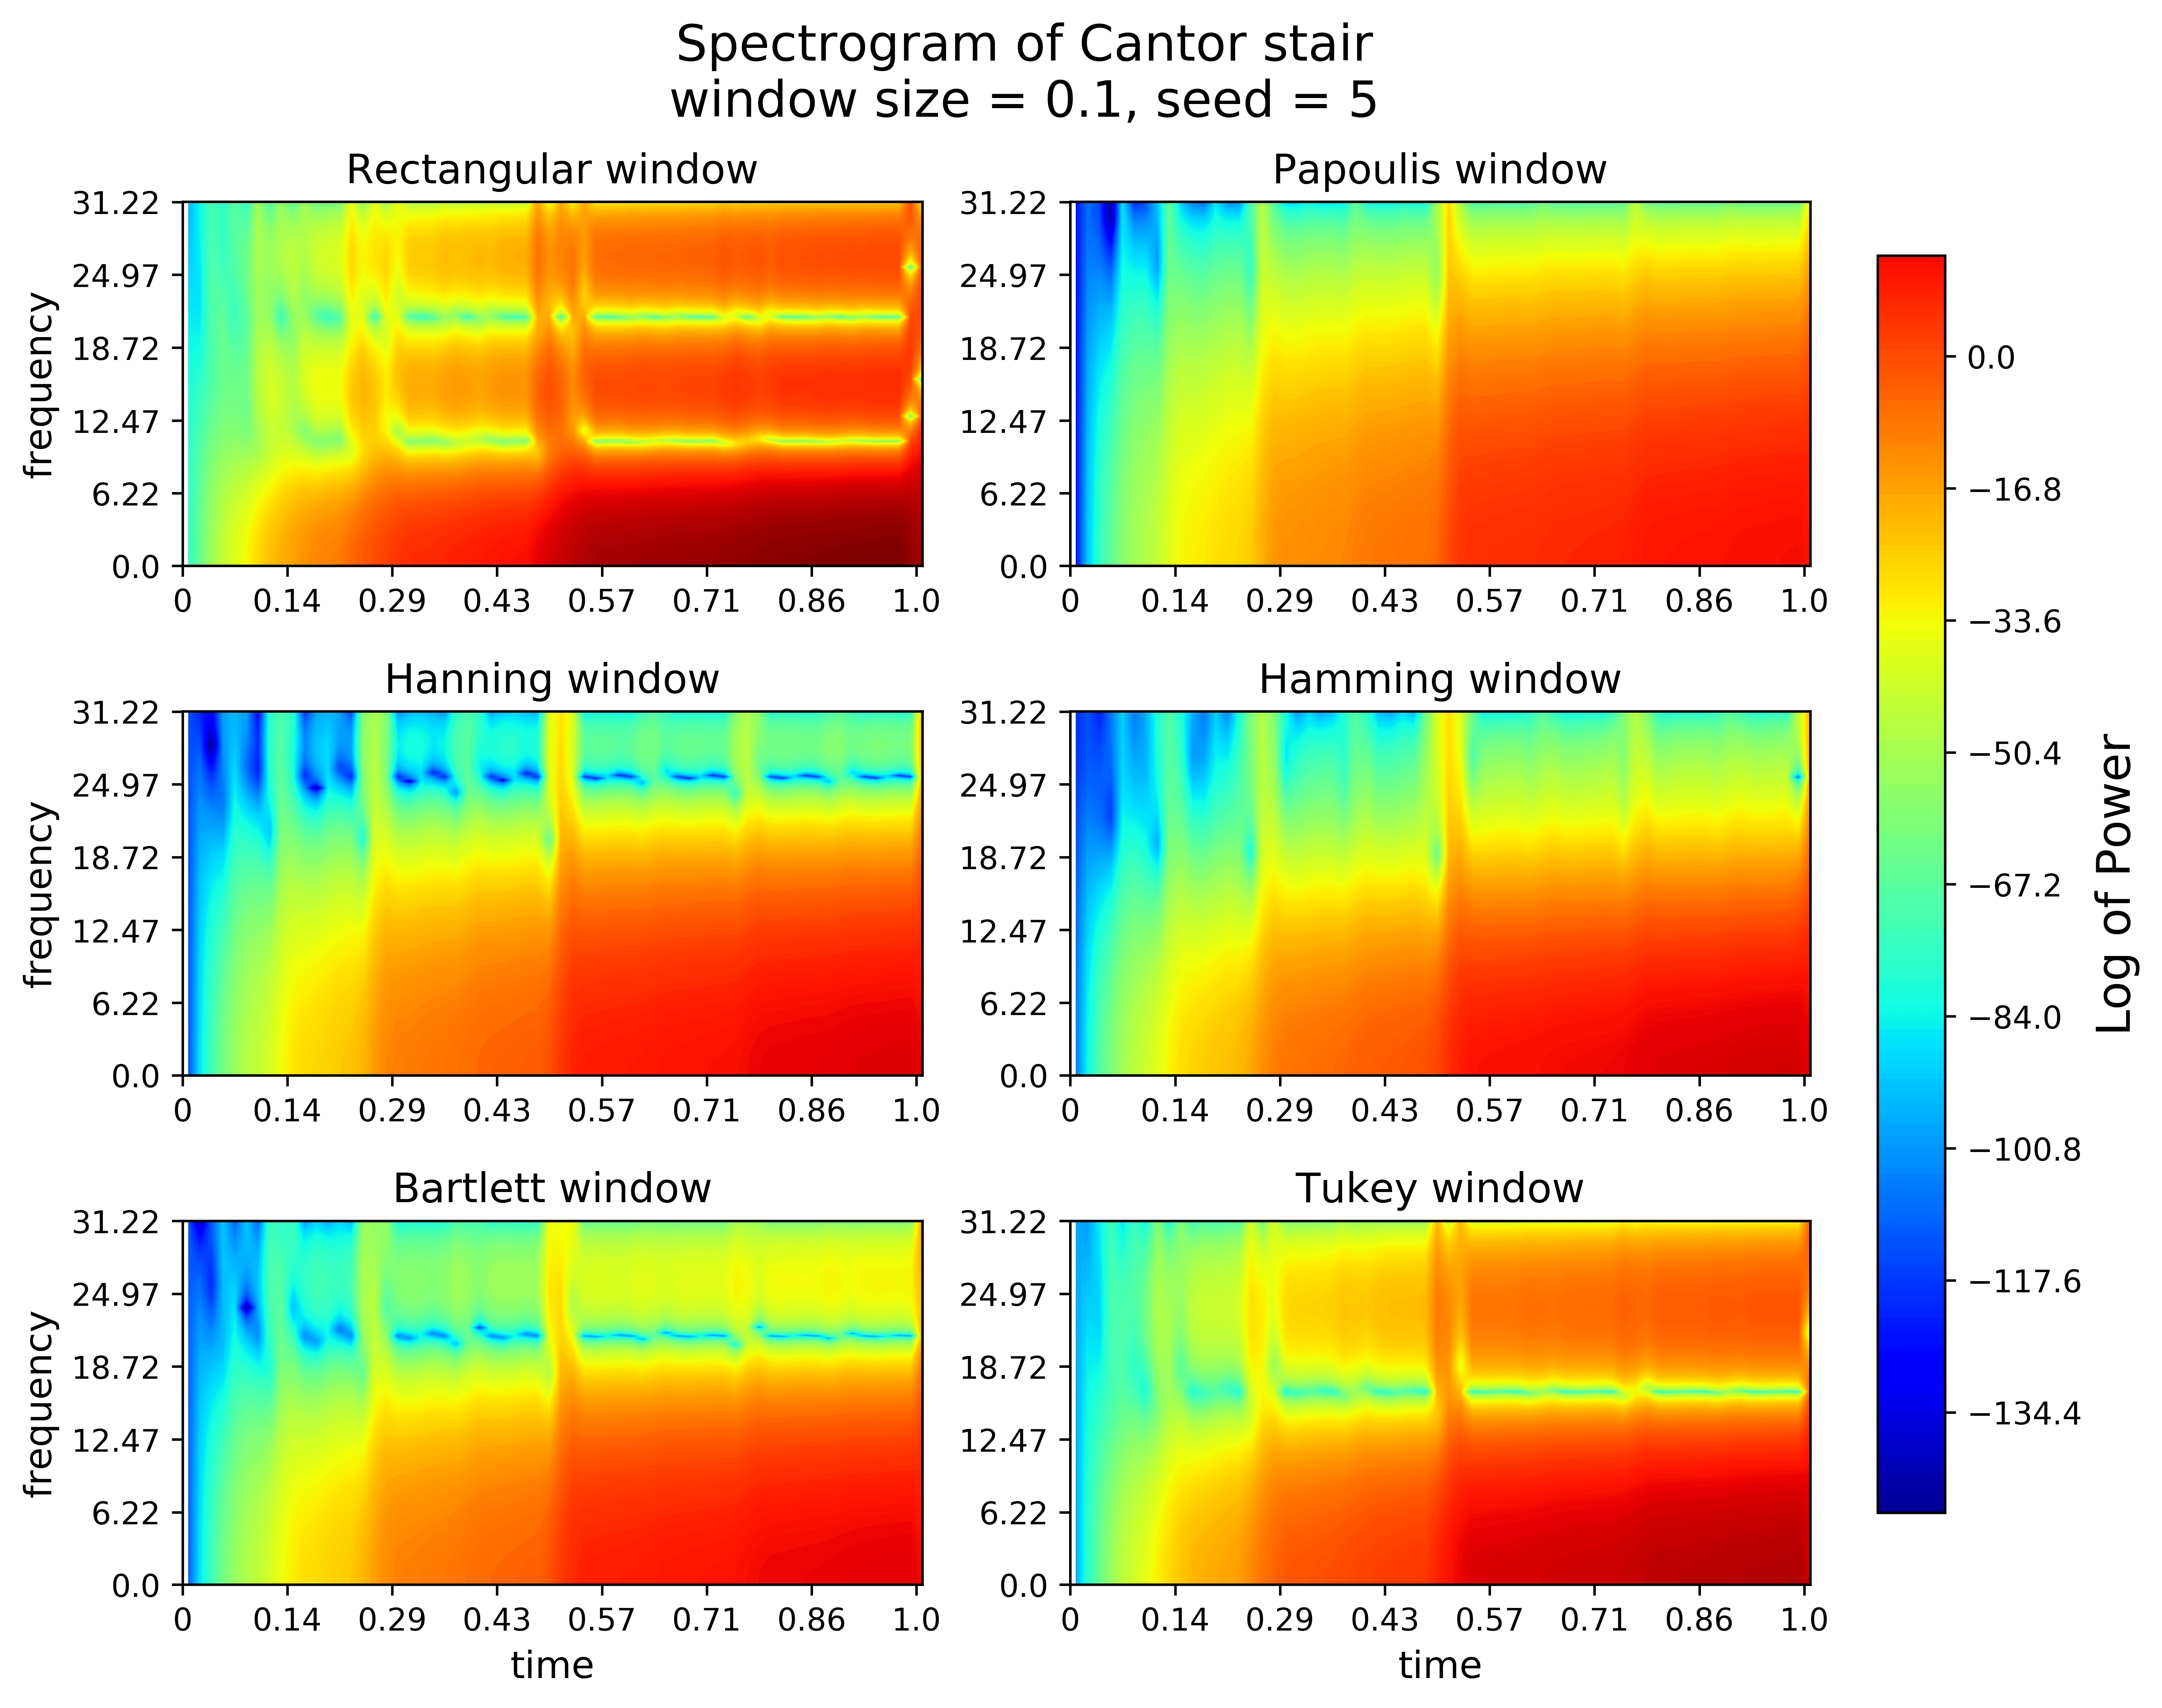
\includegraphics{../Figuras/Cantor stair_seed5_ws0.1.jpg}}
	\end{center}
	\vspace{1mm}	
	\caption{Resultado para \texttt{seed} = 5, tamanho da janela = 0.1. Sob esta configuração, o espectrograma possui maior resolução temporal. Observa-se a partir da janela retangular que existem três momentos em que uma nova gama de frequências é adicionada ao sinal. As demais janelas não obtiveram resultados equivalentes com relação ao nível de informações presentes no espectrograma. Em particular, Papoulis e Hamming obtiveram o pior desempenho. Os três cortes verticais presentes correspondem aos degraus mais altos da função de Cantor (ver Figura \ref{fig:resume}).}
	%\legenda{LEGENDA.} % 	% legenda - para deixar sem legenda usar comando \legenda{} (nunca deve-se comentar o comando \legenda)
	\label{fig:seed5_0.1}
\end{figure}
\begin{figure}[ht!]
	\vspace{1mm}	
	\begin{center}
		\resizebox{15cm}{!}{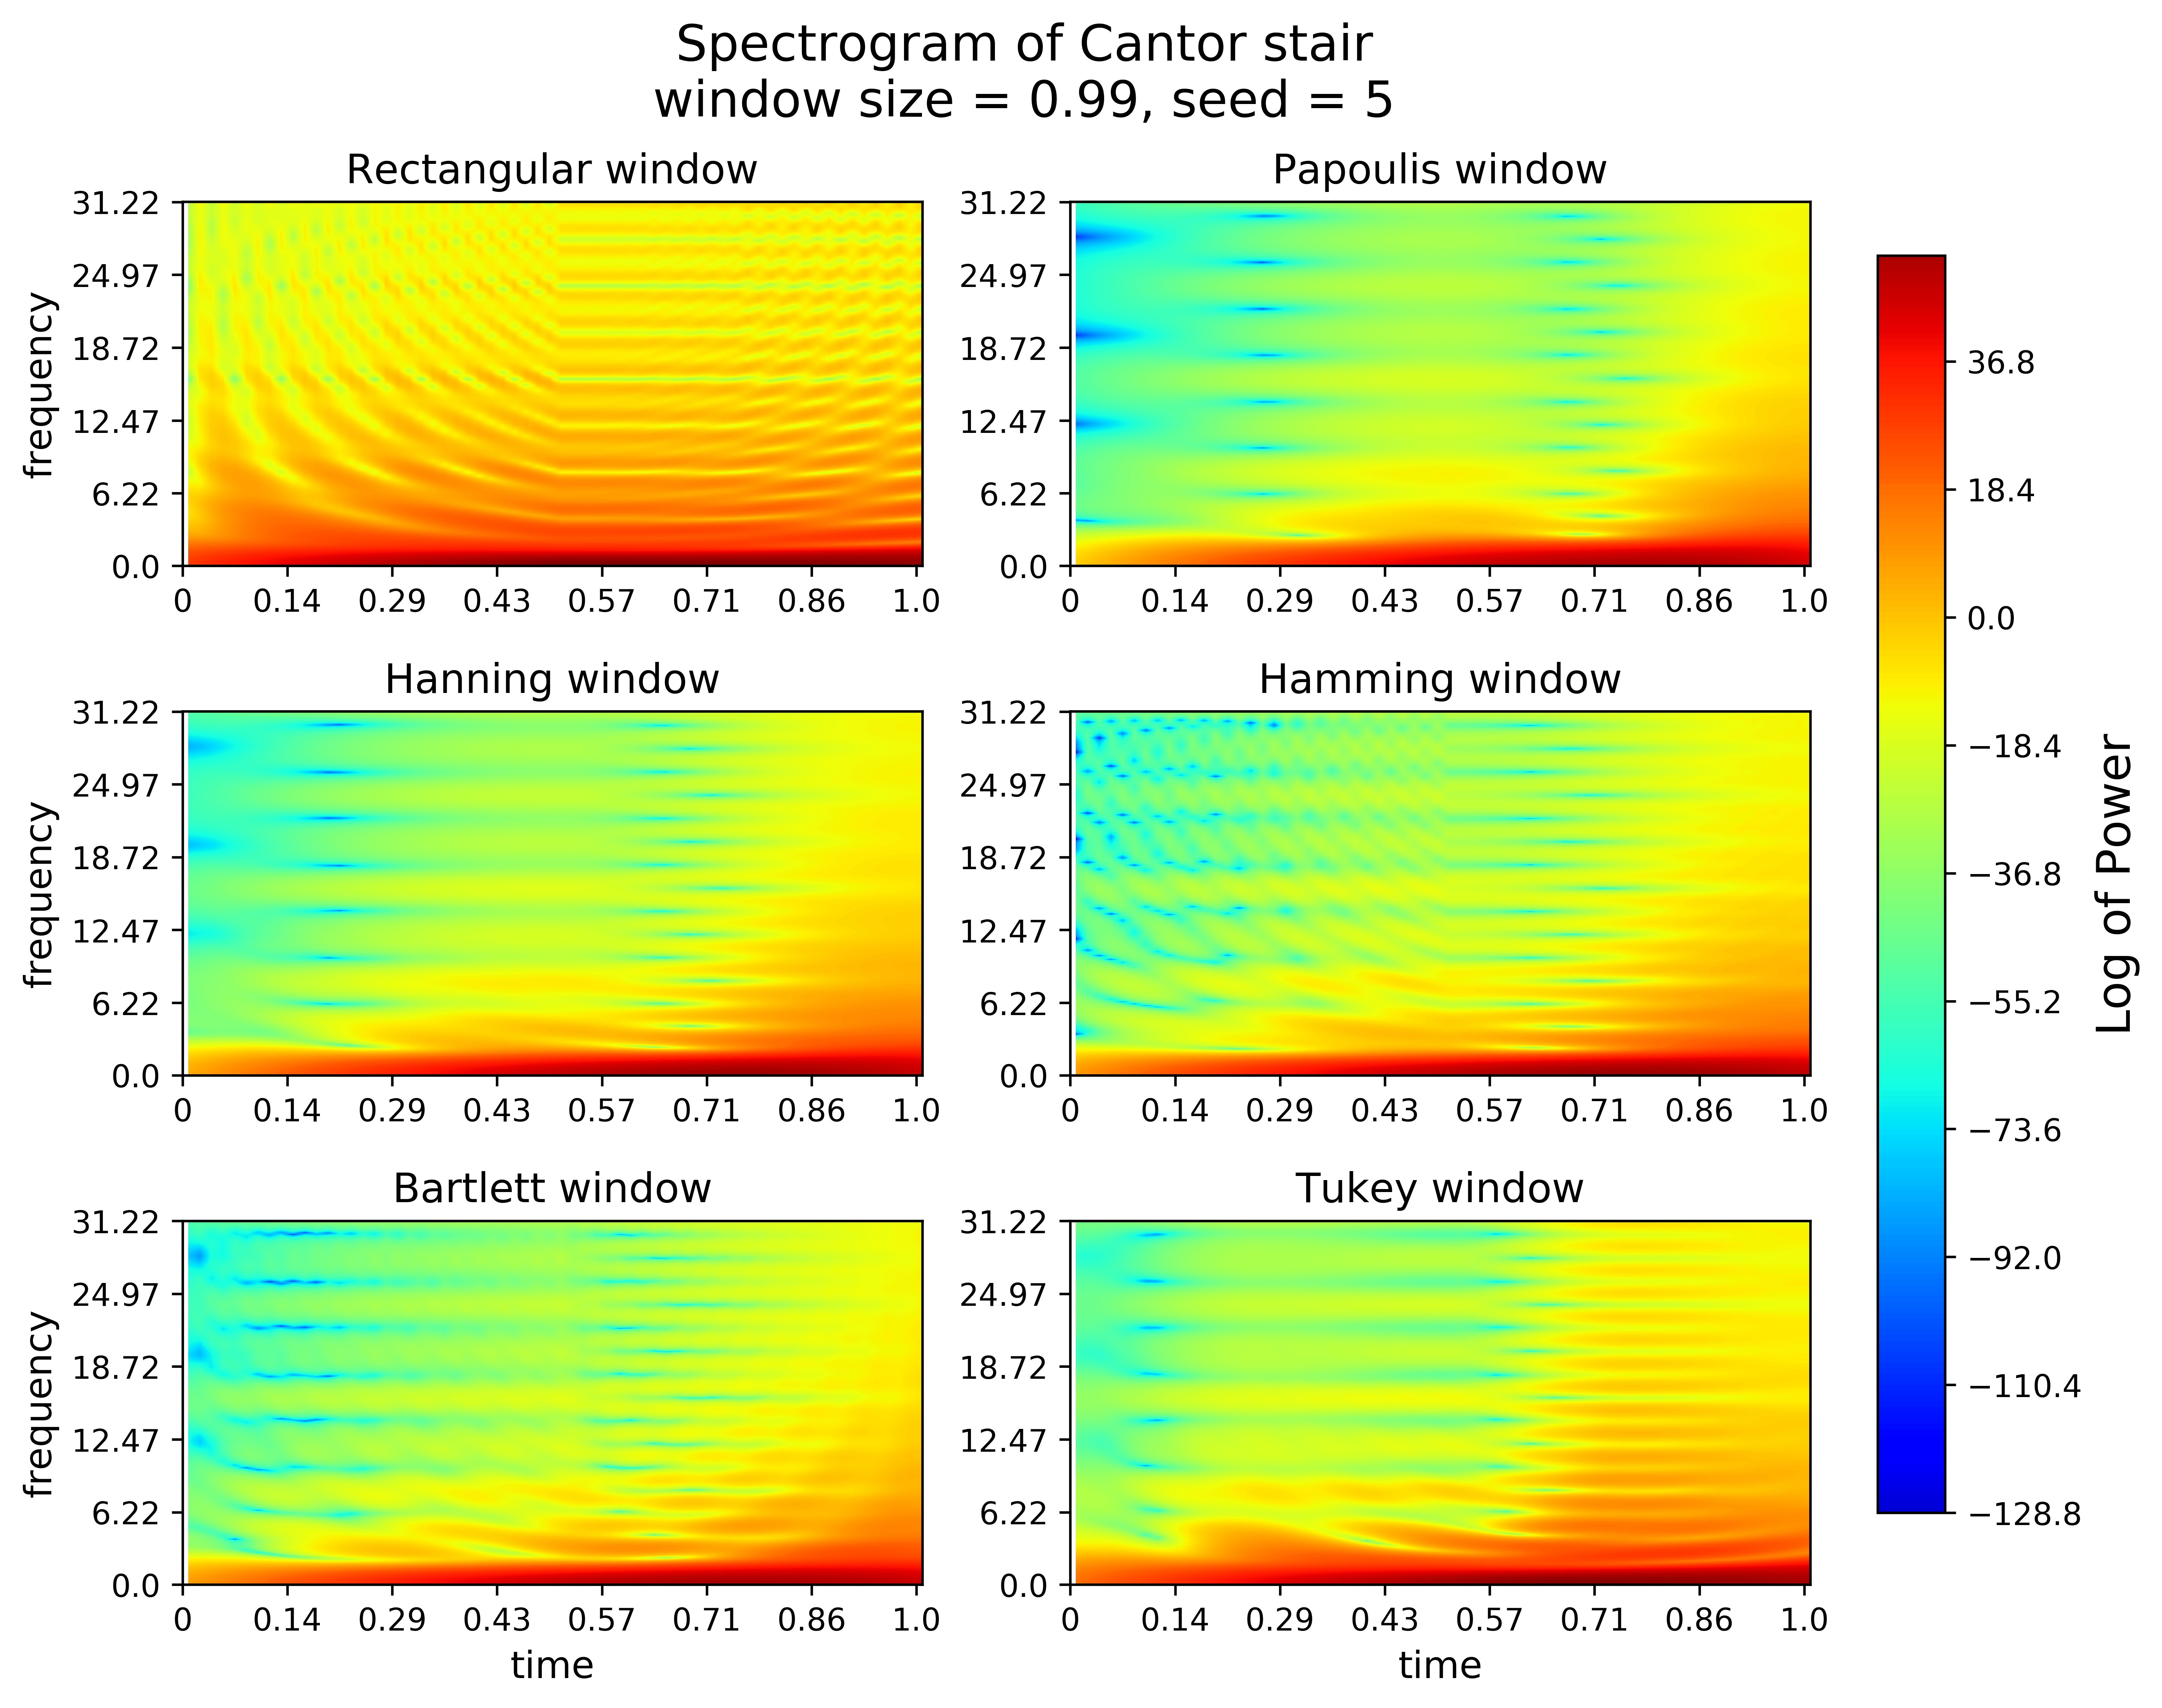
\includegraphics{../Figuras/Cantor stair_seed5_ws0.99.jpg}}
	\end{center}
	\vspace{1mm}	
	\caption{Resultado para \texttt{seed} = 5, tamanho da janela = 0.99. Aqui a resolução da frequência é maior. Observa-se uma assimetria no eixo horizontal: frequências altas dominam a segunda metade dos espectrogramas. Apenas o espectrograma da janela retangular não apresenta essa característica, exibindo detalhes de maneira mais uniforme ao longo do tempo.} 
	% (com exceção da janela retangular). 
	%\legenda{Resultado para \texttt{seed} = 5, tamamho da janela = 0.99. Com uma janela tão grande, a resolução da frequência } % 	% legenda - para deixar sem legenda usar comando \legenda{} (nunca deve-se comentar o comando \legenda)
	\label{fig:seed5_0.99}
\end{figure}

%============================== Seed 7
\begin{figure}[ht!]
	\vspace{1mm}	
	\begin{center}
		\resizebox{15cm}{!}{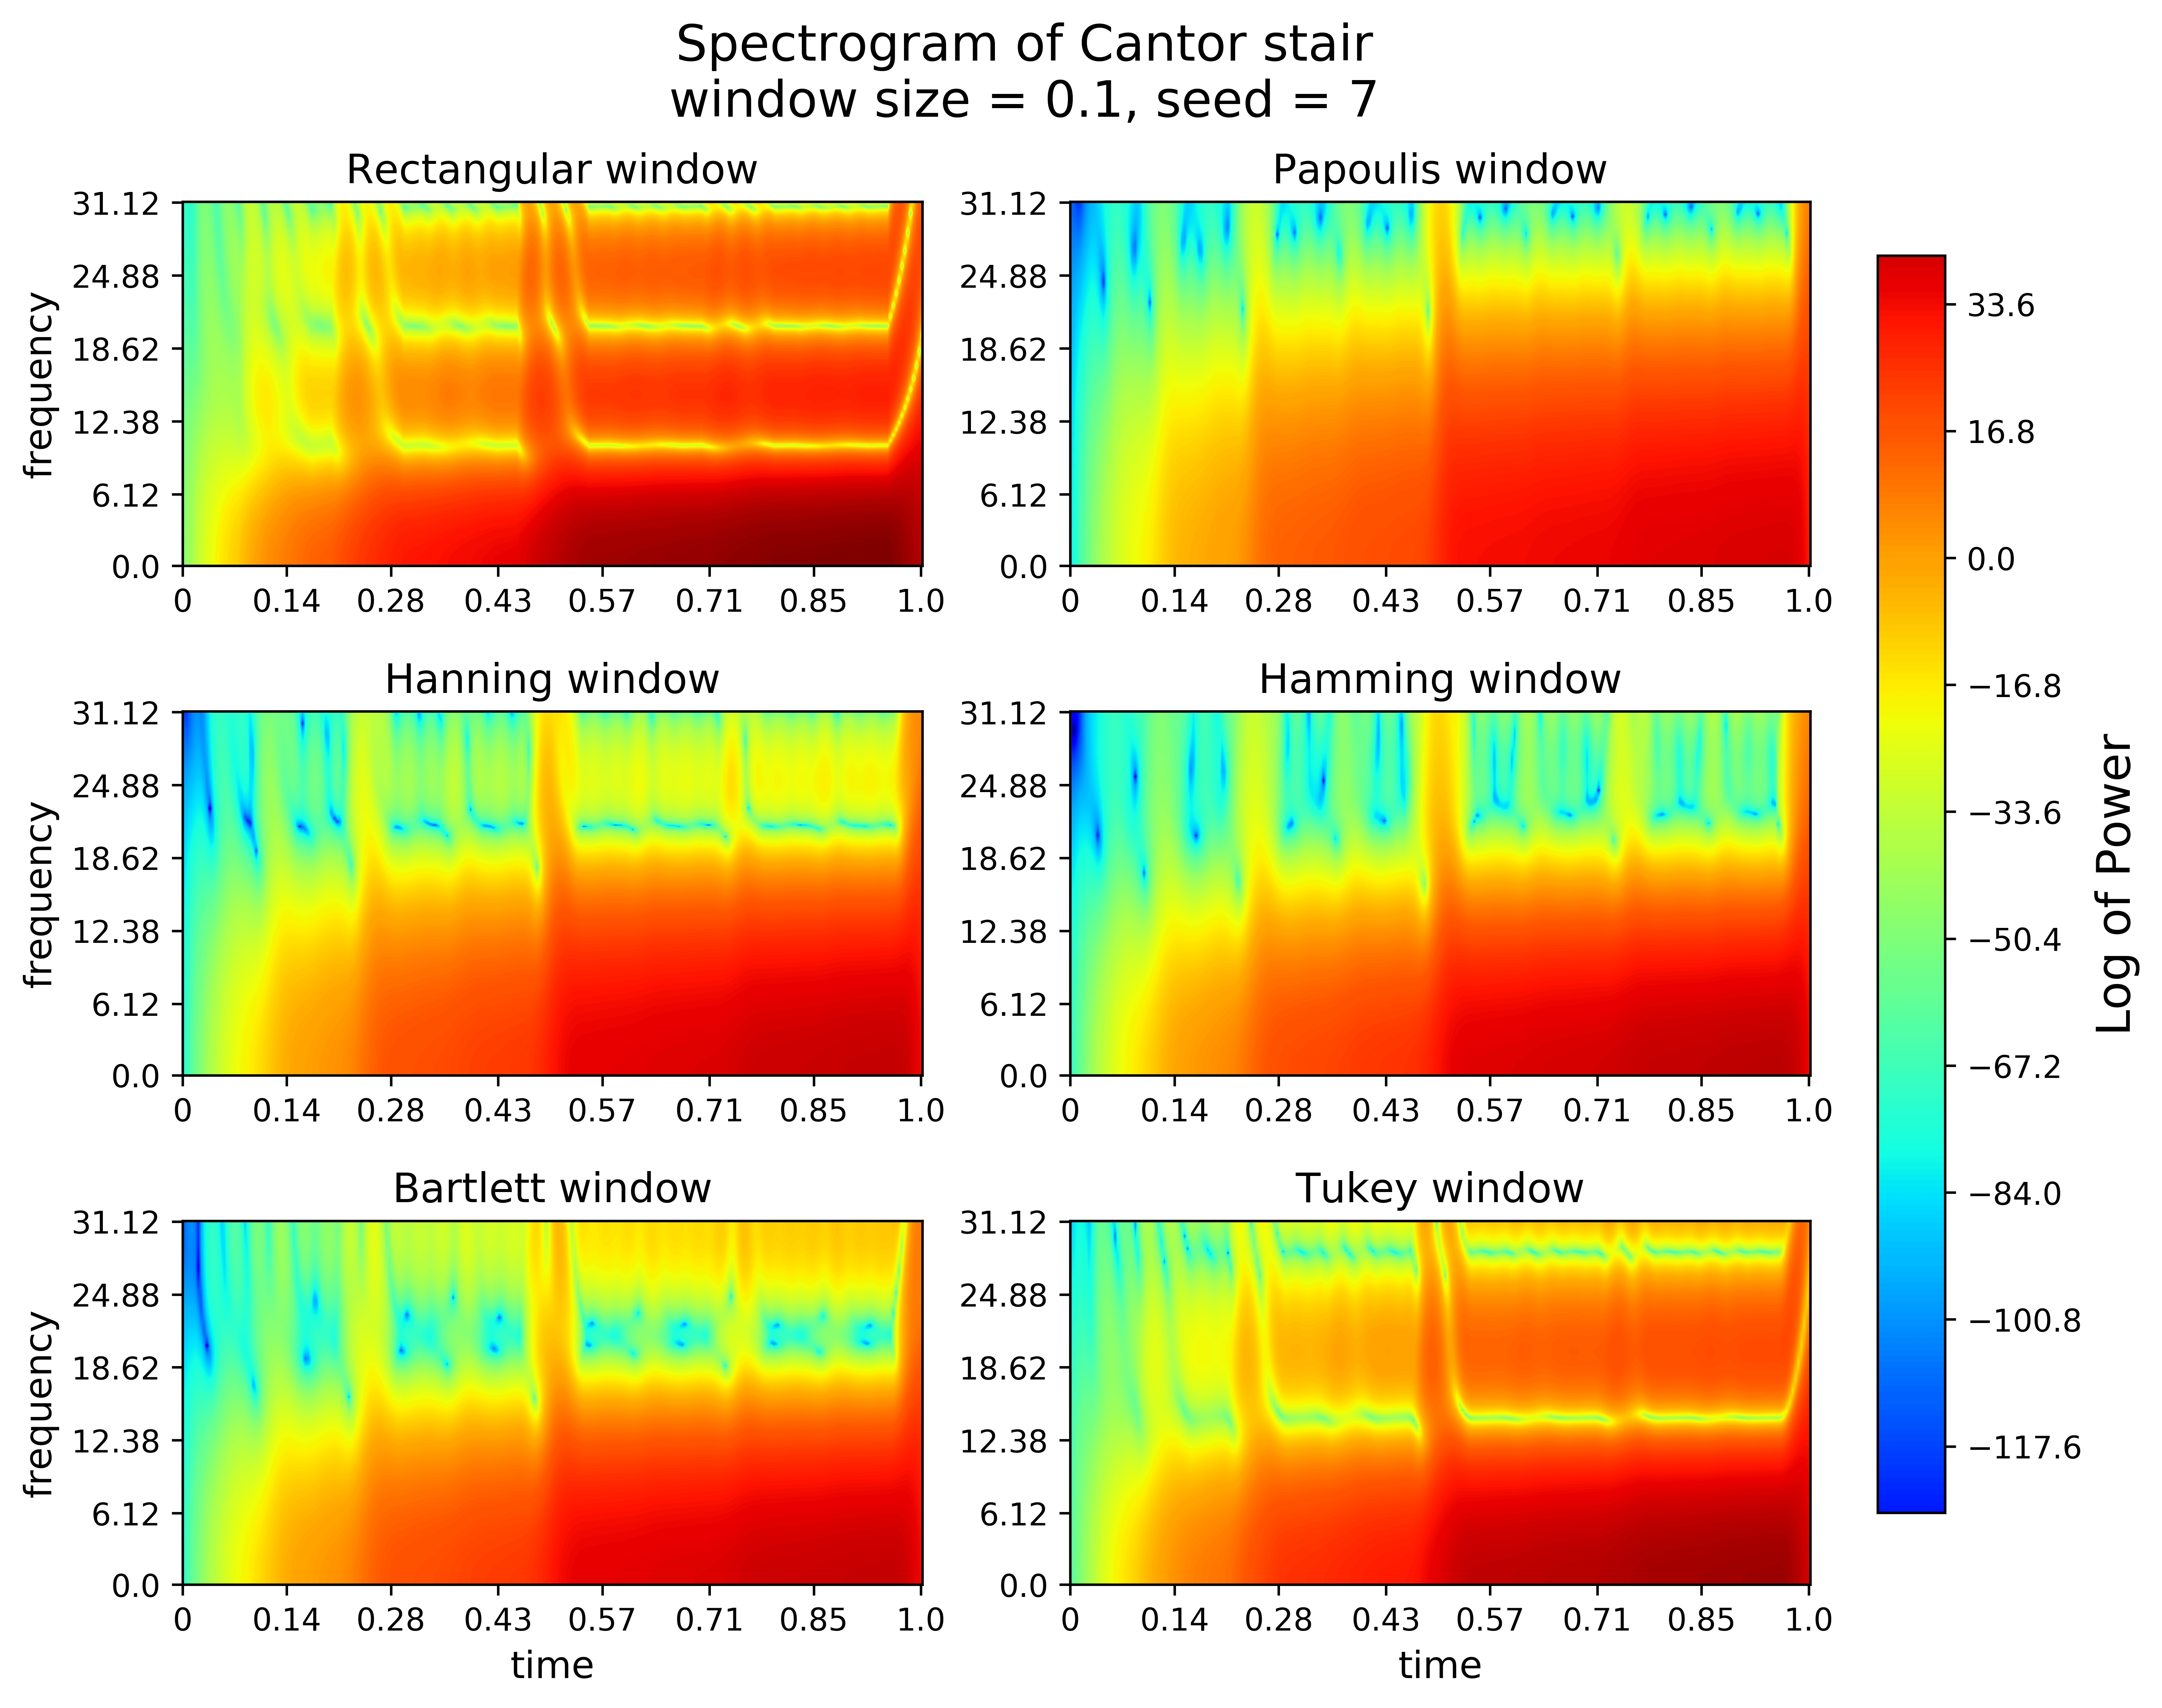
\includegraphics{../Figuras/Cantor stair_seed7_ws0.1.jpg}}
	\end{center}
	\vspace{1mm}	
	\caption{Resultado para \texttt{seed} = 7, tamanho da janela = 0.1. Os espectrogramas exibem maiores cortes verticais quando comparado com a Figura \ref{fig:seed5_0.1}.}
	%\legenda{LEGENDA.} % 	% legenda - para deixar sem legenda usar comando \legenda{} (nunca deve-se comentar o comando \legenda)
	\label{fig:seed7_0.1}
\end{figure}
\begin{figure}[ht!]
	\vspace{1mm}	
	\begin{center}
		\resizebox{15cm}{!}{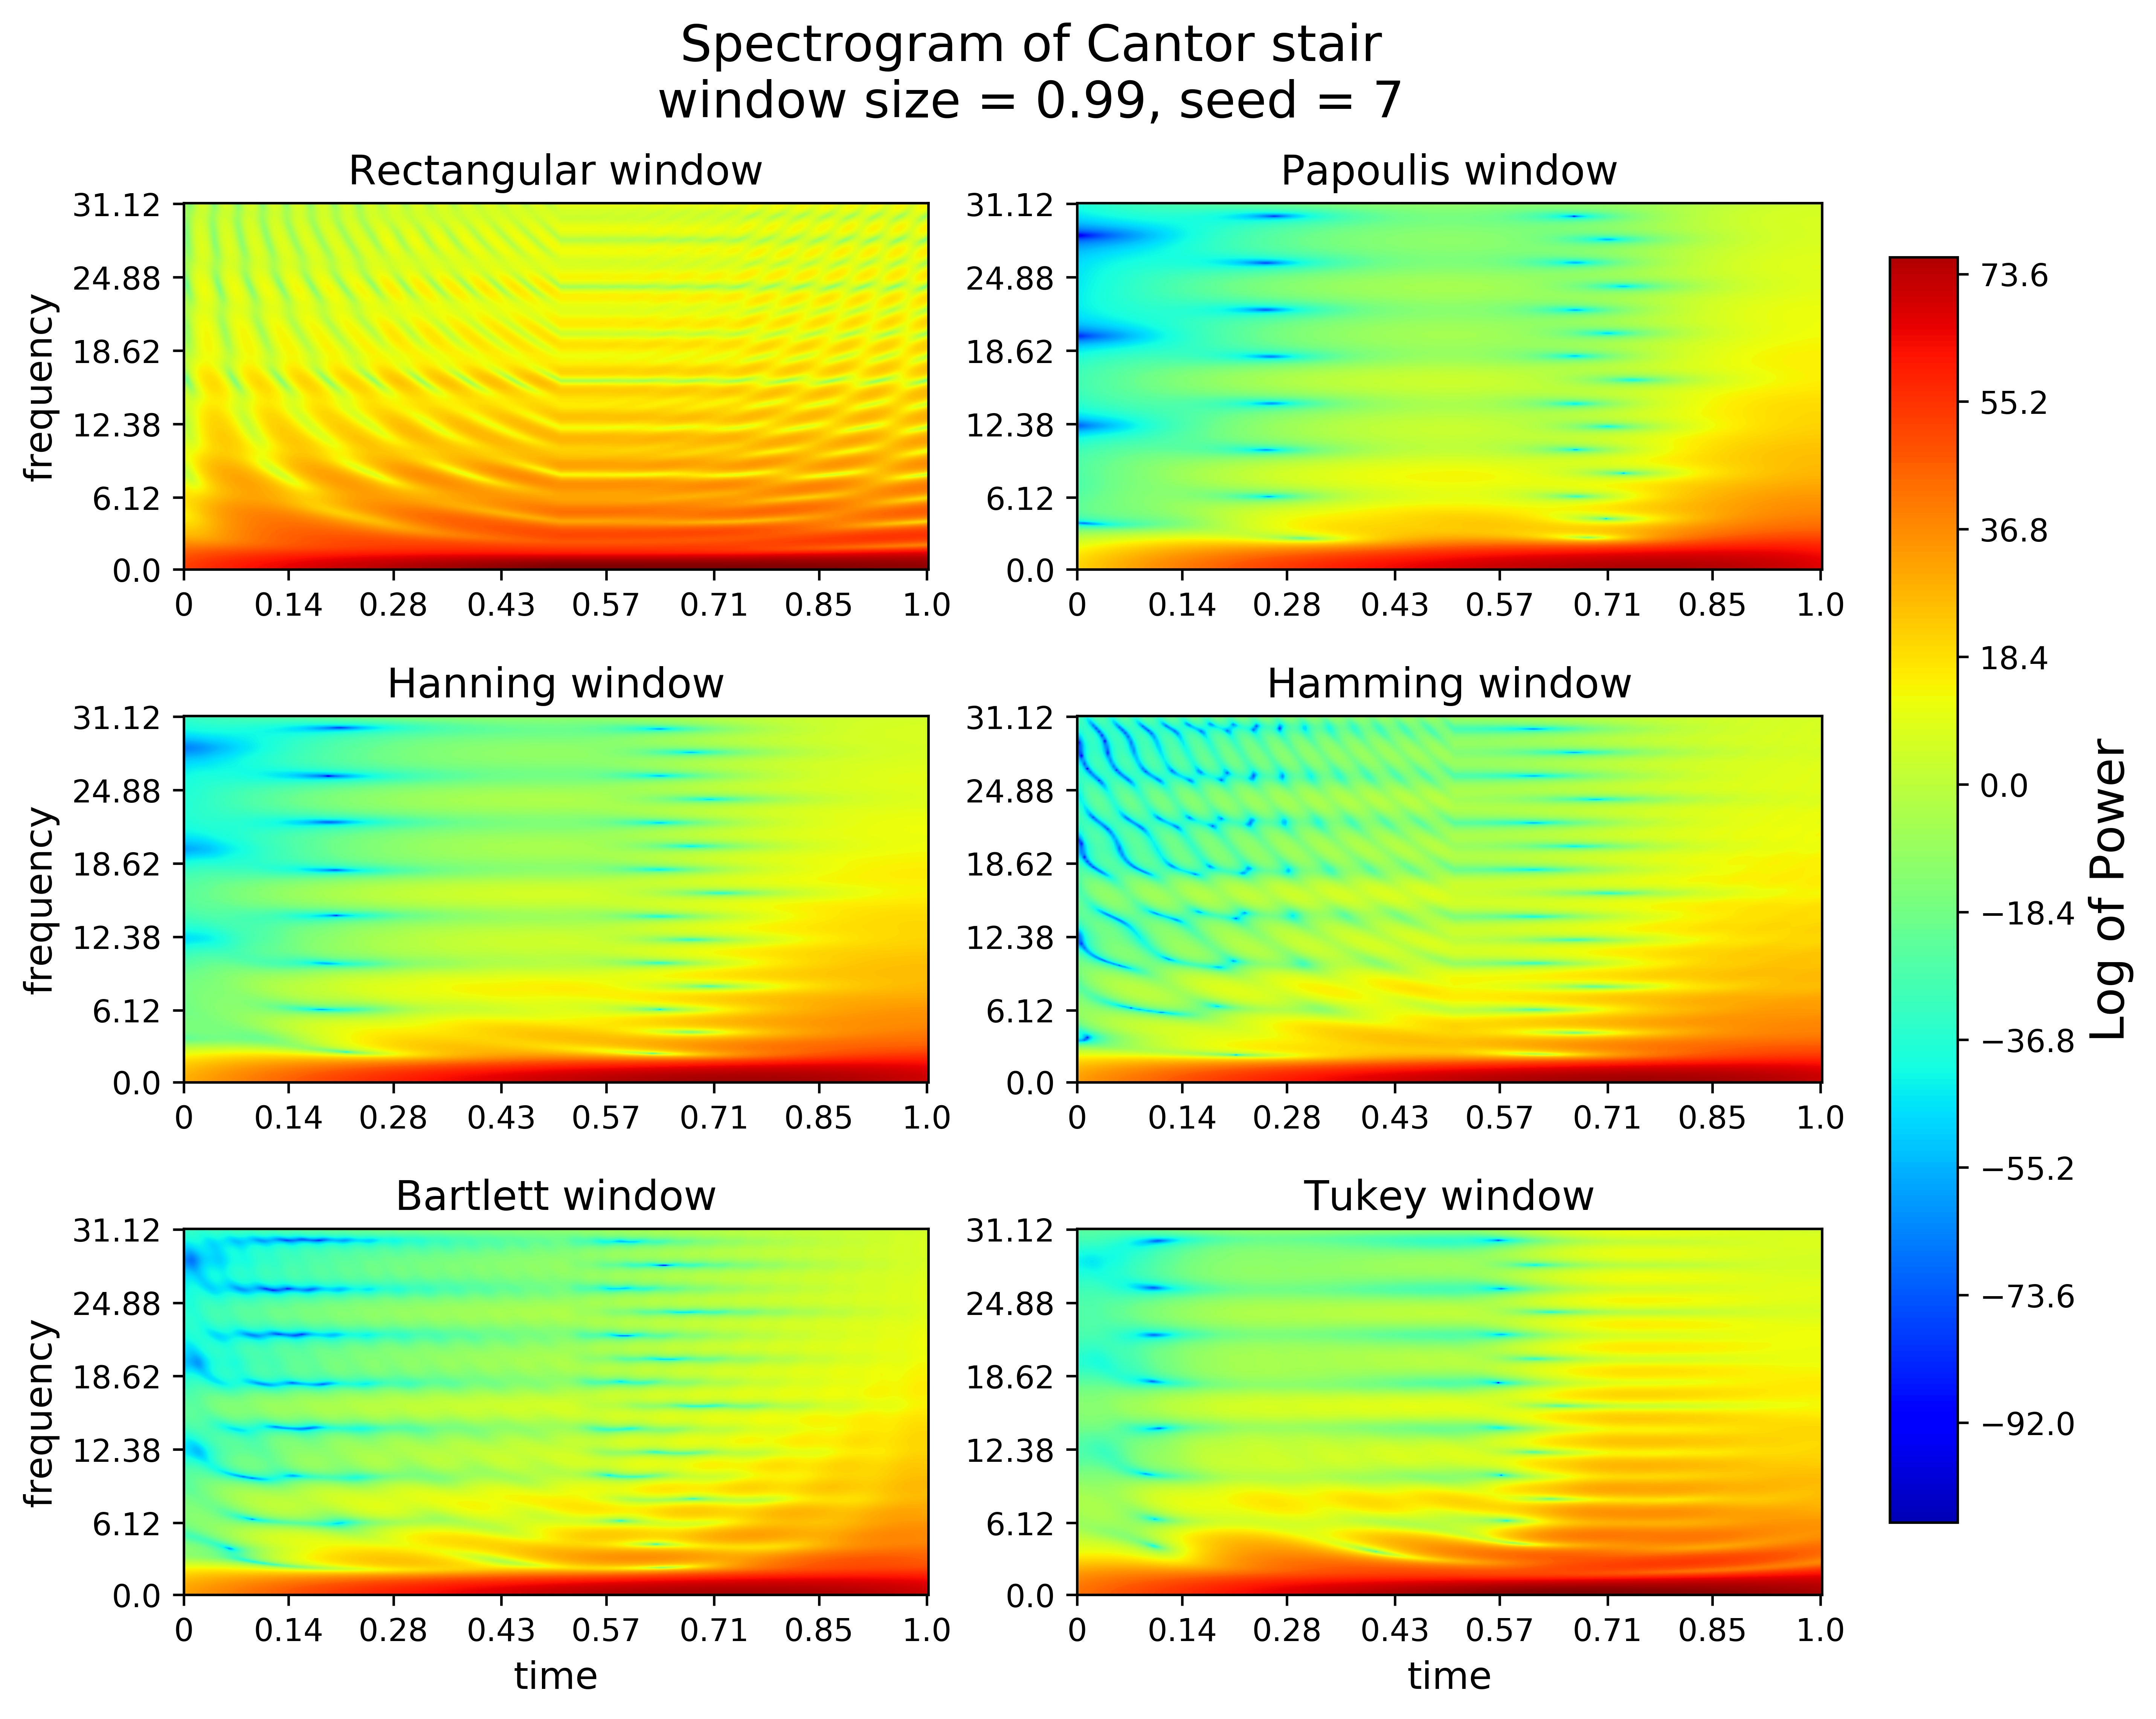
\includegraphics{../Figuras/Cantor stair_seed7_ws0.99.jpg}}
	\end{center}
	\vspace{1mm}	
	\caption{Resultado para \texttt{seed} = 7, tamanho da janela = 0.99. A mesma assimetria da Figura \ref{fig:seed5_0.99} é observada.} 
	%\legenda{LEGENDA.} % 	% legenda - para deixar sem legenda usar comando \legenda{} (nunca deve-se comentar o comando \legenda)
	\label{fig:seed7_0.99}
\end{figure}


%============================== Seed 10
\begin{figure}[ht!]
	\vspace{1mm}
	\begin{center}
		\resizebox{15cm}{!}{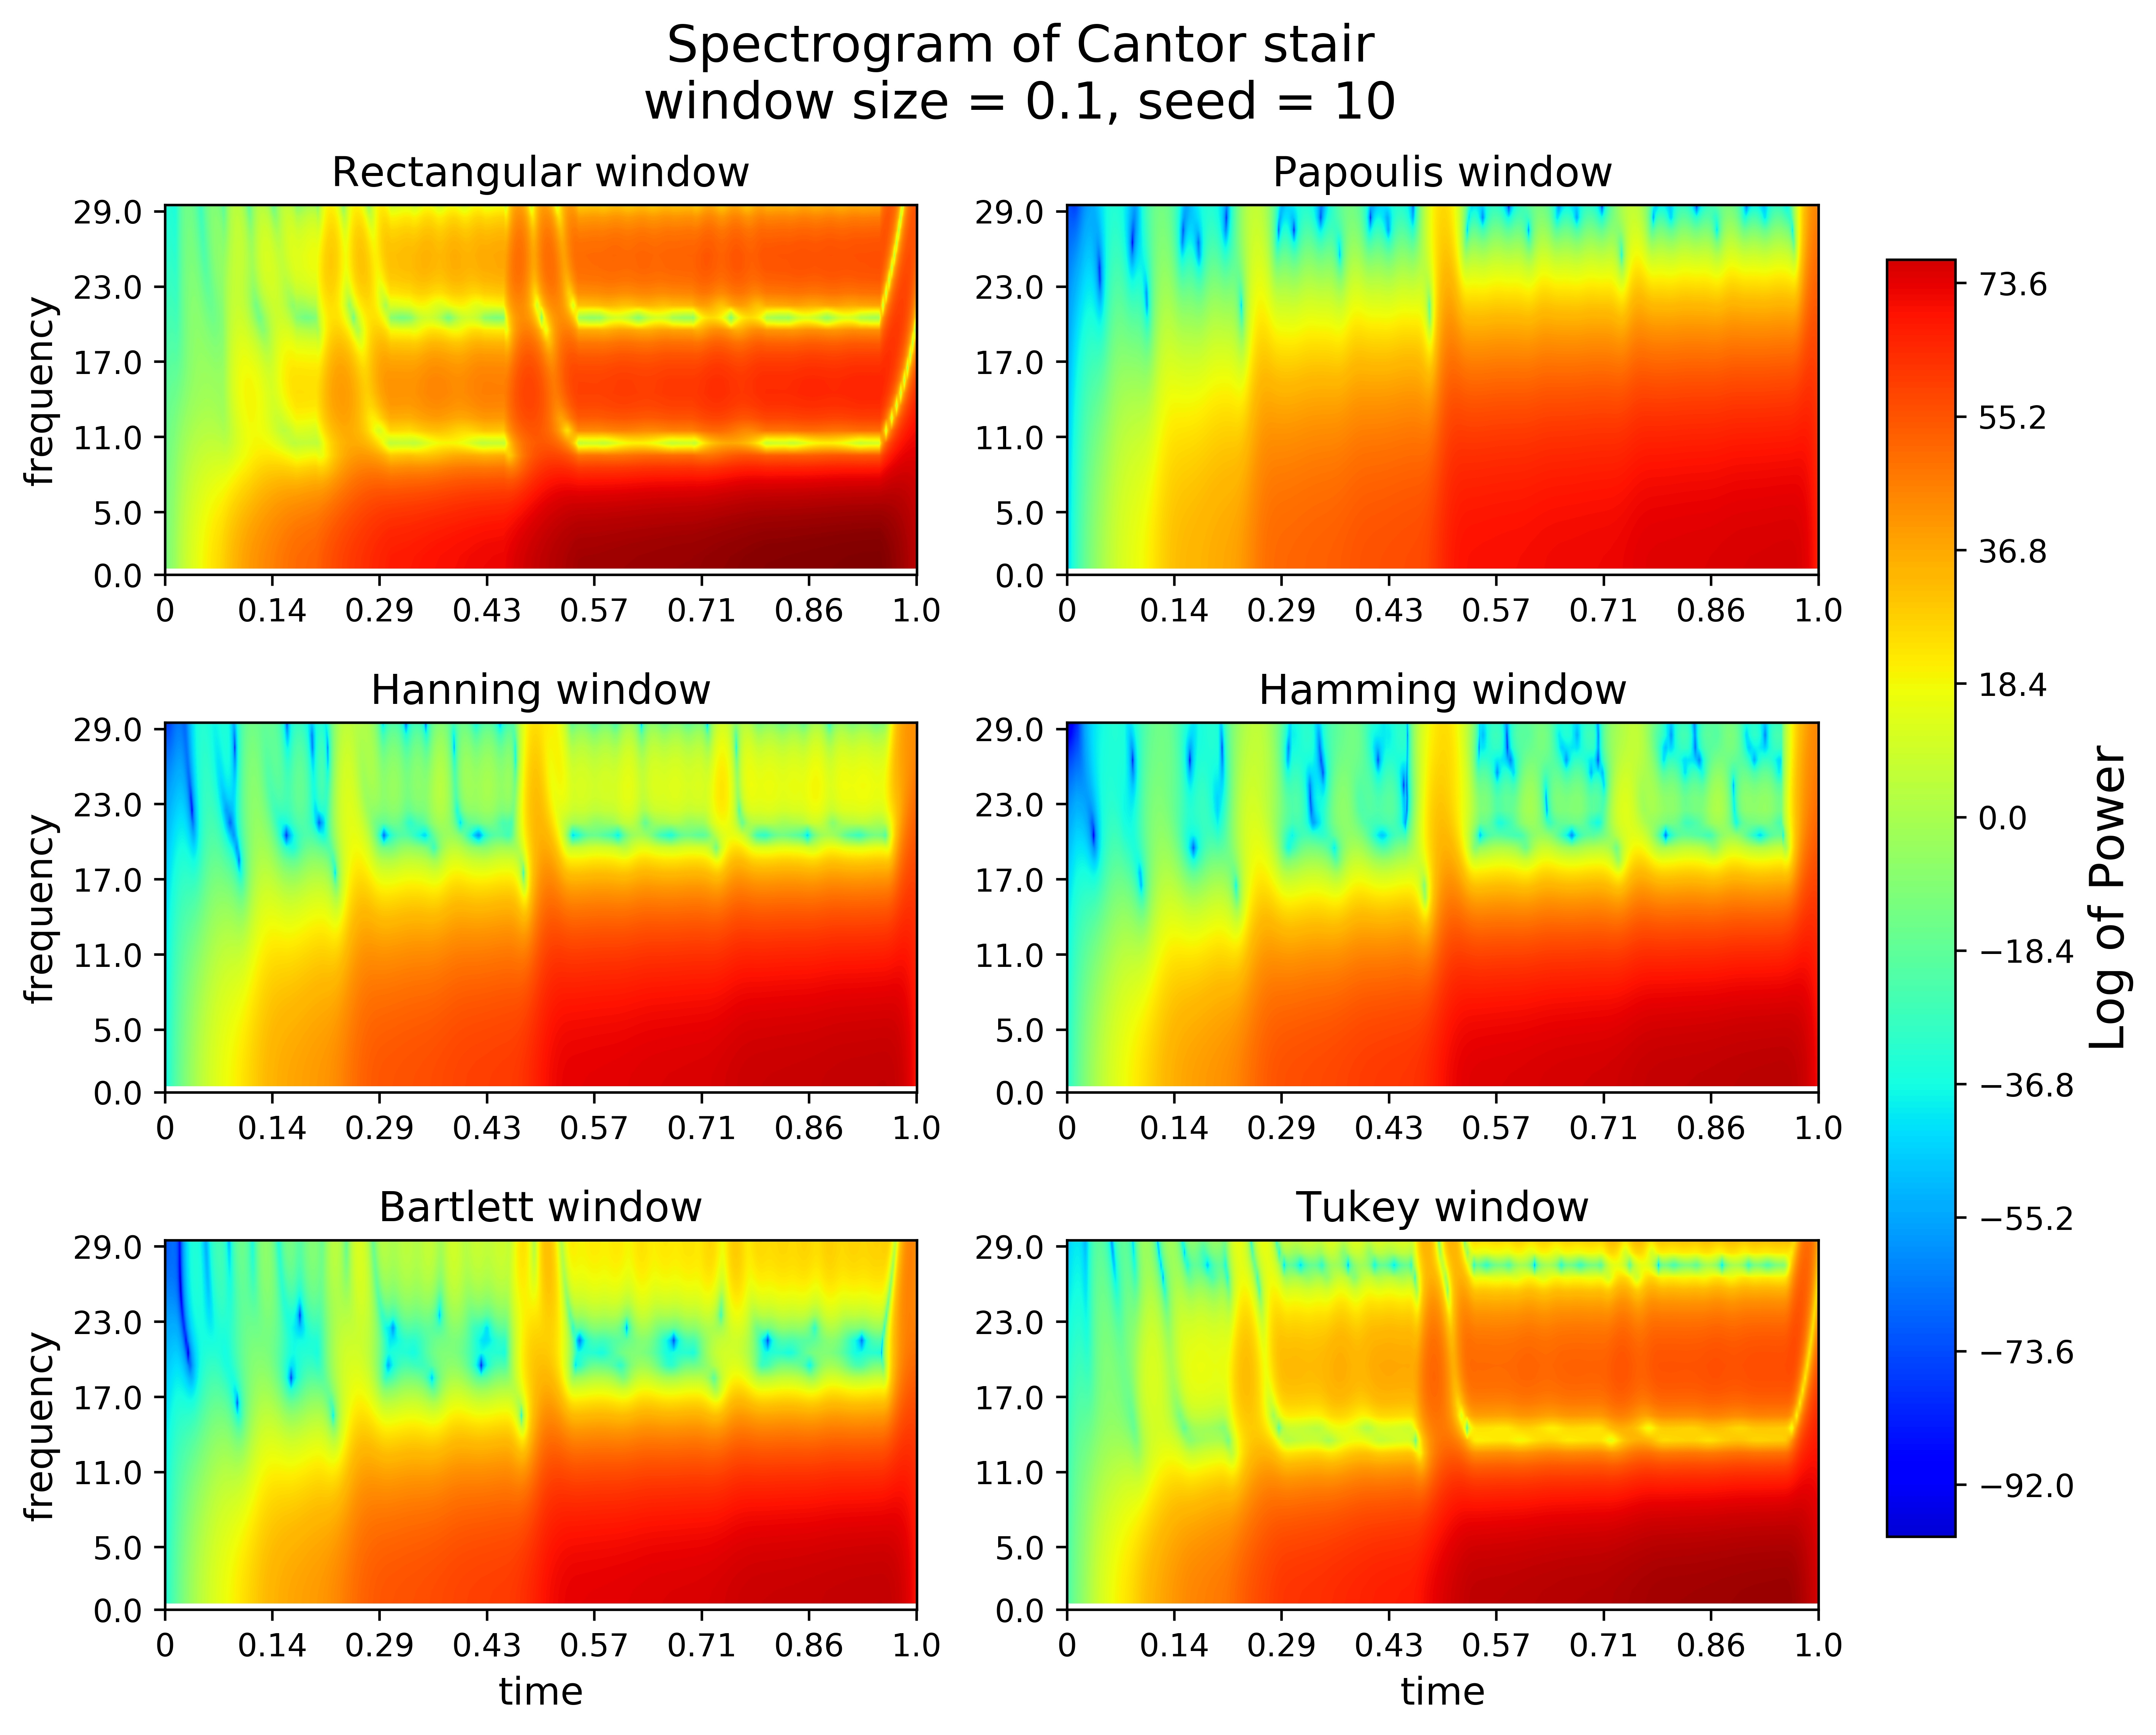
\includegraphics{../Figuras/Cantor stair_seed10_ws0.1.jpg}}
	\end{center}
	\vspace{1mm}
	\caption{Resultado para \texttt{seed} = 10, tamanho da janela = 0.1. Novamente a janela retangular foi capaz de captar melhor os momentos em que altas frequências são introduzidas. Os cortes verticais estão mais proeminentes.}
	%\legenda{LEGENDA.} 	% legenda - para deixar sem legenda usar comando \legenda{} (nunca deve-se comentar o comando \legenda)
	\label{fig:seed10_0.1}
\end{figure}
\begin{figure}[ht!]
	\vspace{1mm}	
	\begin{center}
		\resizebox{15cm}{!}{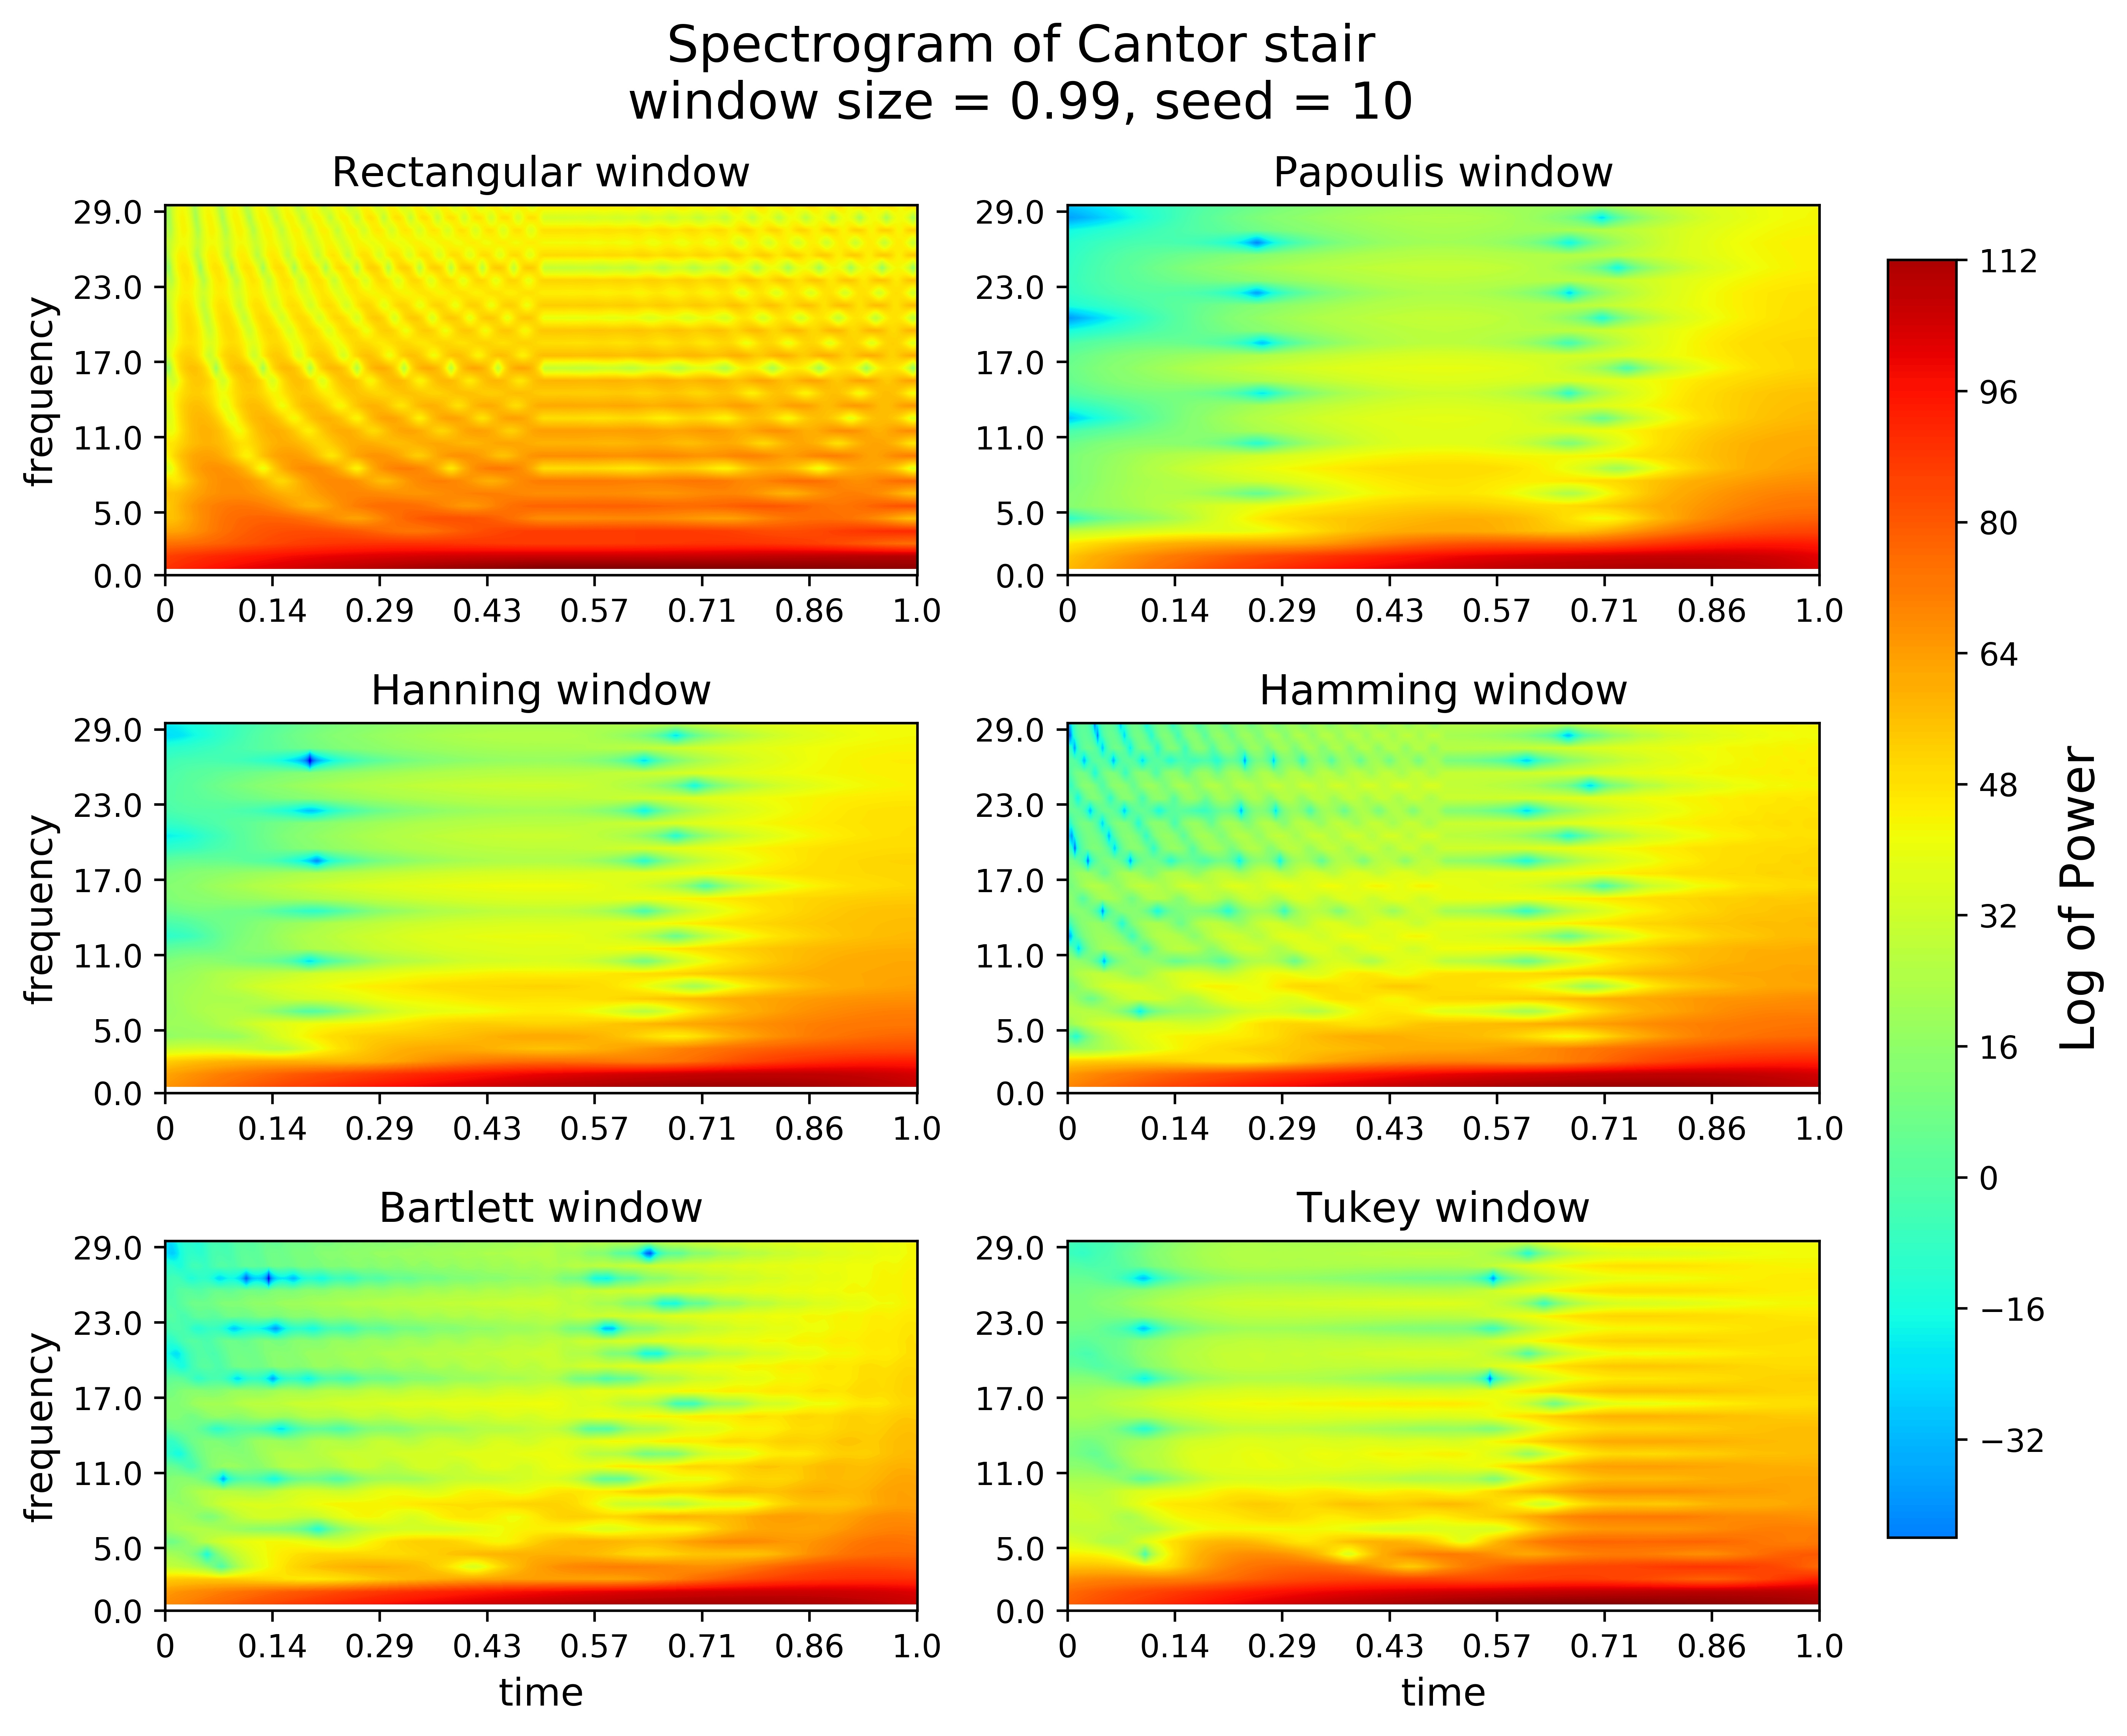
\includegraphics{../Figuras/Cantor stair_seed10_ws0.99.jpg}}
	\end{center}
	\vspace{1mm}
	\caption{Resultado para \texttt{seed} = 10, tamanho da janela = 0.99. O espectrogram apresenta mais energia que os demais e ainda mais detalhe de frequência.}
	%\legenda{LEGENDA.} % 	% legenda - para deixar sem legenda usar comando \legenda{} (nunca deve-se comentar o comando \legenda)
	\label{fig:seed10_0.99}
\end{figure}